\documentclass[11pt]{article}
\usepackage[preprint]{acl}

\usepackage{times}
\usepackage{latexsym}
\usepackage[T1]{fontenc}
\usepackage[utf8]{inputenc}
\usepackage{microtype}
%\usepackage{inconsolata}
\usepackage{graphicx}
\usepackage{booktabs}
\usepackage{amsmath}
\usepackage{multirow}

\title{Indistinguishable at the Top: A Statistical Audit of the\\
       BLP-2025 Bangla Hate Speech Shared Task}

\author{Gazi Shoaib \\
  Jahangirnagar University \\
  Savar, Dhaka, Bangladesh \\
  \texttt{gazishoaib953@gmail.com}}

\begin{document}
\maketitle

\footnotetext[1]{Code and analysis scripts:
\texttt{github.com/gazishoaib33/blp25-audit}}
\renewcommand{\thefootnote}{\arabic{footnote}}

\begin{abstract}
Shared-task leaderboards routinely report scores to four decimal places and rank
systems accordingly, but rarely report whether those ranks are distinguishable
from noise. We audit the BLP-2025 Bangla Hate Speech Identification shared task,
whose data, gold test labels, and evaluation scripts are fully public. We find
that in all three subtasks the top five systems are statistically
indistinguishable: the top-five spread is 0.34--0.80 percentage points against a
95\% confidence interval half-width of 0.85--0.86 points, and for the
leader-versus-runner-up gap to reach $p<.05$ under McNemar's test the two systems
would have to disagree on under 1.2\% of test items. We then test, and reject,
the hypothesis that annotation noise caps performance: three-way majority voting
over annotations with $\kappa=0.71$ yields gold labels we estimate to be
$\approx$97\% reliable, leaving a 24-point gap to the best system. The binding
problem is instead the metric. Because \textsc{Sexism} comprises 29 of 10{,}200
test items, a system that detects every sexist comment and one that detects none
differ by 0.28 points of micro-F1---below the 0.44-point sampling noise floor.
Training ten systems to obtain real predictions, we measure pairwise discordance
of 3.6--36.3\% and show that the minimum detectable gap is 0.37\,pp even in the
best case---above every reported top-two gap---while a pair separated by
0.02\,pp wins only 51.5\% of bootstrap resamples. No system in our pool detects
more than 3 of the 29 sexist comments, and five detect none. All analysis code is
released.
\end{abstract}

\section{Introduction}
\label{sec:intro}

A shared task converts a research question into a ranking. The ranking is what
participants optimise, what system-description papers narrate, and what
subsequent work cites as the state of the art. Yet the NLP community has known
for some time that small score differences on a fixed test set are frequently
indistinguishable from sampling noise
\citep{reimers2017reporting,dror2018hitchhiker,card2020power}, and that
benchmarks themselves carry label errors that destabilise the orderings they
induce \citep{northcutt2021labelerrors,bowman2021benchmarking}.

\citet{jin2026broken} recently applied this scrutiny to text-to-SQL, manually
re-examining two widely used benchmarks and reporting annotation error rates of
52.8\% and 66.1\%. Their central observation is not that any single benchmark is
bad but that \emph{nobody had checked}. We ask the same question of a
low-resource benchmark, where the stakes are arguably higher: resources are
scarcer, so a single shared task shapes a larger fraction of subsequent work.

We audit BLP-2025 Task 1, Bangla Hate Speech Identification
\citep{hasan2025blptask1}, a well-run shared task that attracted over 160
participants and---critically for our purposes---released its data, its gold test
labels, and its scorer. Our contributions:

\begin{enumerate}\itemsep2pt
\item In all three subtasks the reported top five are statistically
      indistinguishable (\S\ref{sec:rankings}).
\item We estimate the annotation ceiling from the reported inter-annotator
      agreement and \emph{reject} the hypothesis that label noise explains the
      observed 0.736 plateau (\S\ref{sec:ceiling}).
\item We show that micro-F1 on this label distribution is formally incapable of
      registering performance on the \textsc{Sexism} class
      (\S\ref{sec:metric}).
\item We identify 342 test items whose labels are internally inconsistent
      (\S\ref{sec:coherence}).
\end{enumerate}

We stress that the dataset survives our integrity checks well
(\S\ref{sec:coherence}), and that this audit was only possible \emph{because}
the organisers released everything needed to run it.

\section{Related Work}

\paragraph{Significance in NLP.} \citet{reimers2017reporting} showed that single-run score comparisons are unreliable; \citet{dror2018hitchhiker} surveyed
appropriate tests; \citet{card2020power} demonstrated that many NLP experiments
are badly underpowered for the effect sizes they claim. Our
\S\ref{sec:rankings} applies this lens to a shared-task leaderboard rather than
to a single paper's ablations.

\paragraph{Benchmark quality.} \citet{northcutt2021labelerrors} found pervasive
label errors across ten popular test sets and showed that correcting them
reorders model rankings; \citet{jin2026broken} performed the analogous audit for
text-to-SQL. \citet{vidgen2020directions} survey quality problems specific to
abusive-language corpora, and \citet{sap2019racialbias} show how annotation
artifacts translate into deployed bias. We inherit the methodology of
\citet{jin2026broken} while closing a gap in it: that work reports neither an
annotator count, an agreement statistic, nor an adjudication protocol.

\paragraph{Bangla NLP.} Resources for Bangla have expanded rapidly
\citep{bhattacharjee2022banglabert}, and the BLP workshop series has become the
field's principal venue \citep{hasan2025blptask1,raihan2025blptask2}. To our
knowledge no Bangla benchmark has previously been subjected to a quantitative
audit.

\section{The Shared Task}
\label{sec:task}

BLP-2025 Task 1 \citep{hasan2025blptask1} released \textsc{BanglaMultiHate},
50{,}746 YouTube comments from a Bangla news channel spanning 19 topics,
annotated by 35 native speakers with three independent labels per item resolved
by majority vote. Reported Fleiss' $\kappa$ \citep{fleiss1971} is 0.71 for hate
type, 0.79 for target, and 0.84 for severity. Splits are 35{,}522 train /
2{,}512 dev / 2{,}512 dev-test / 10{,}200 test. Three subtasks are evaluated by
micro-F1: 1A predicts hate type (6 classes), 1B target (5 classes), and 1C all
three dimensions jointly.

\paragraph{A reproducibility hazard.} The literal string \texttt{None} is the
majority class (56.4\% of 1A), and \texttt{pandas.read\_csv} silently coerces it
to \texttt{NaN} by default---a trap we hit ourselves. Loads must pass
\texttt{keep\_default\_na=False}; the majority baseline should then reproduce the
organisers' reported 0.5638, which ours does exactly.

\begin{figure*}[t]
\centering
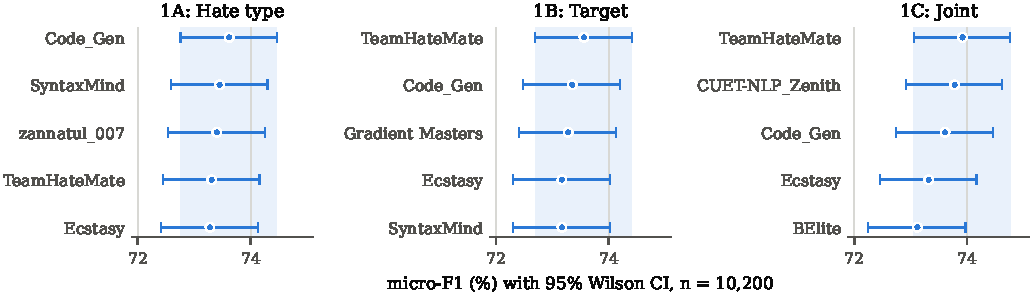
\includegraphics[width=\textwidth]{fig1_leaderboard.pdf}
\caption{Reported micro-F1 for the top five teams in each subtask, with 95\%
Wilson confidence intervals at $n=10{,}200$. In every subtask, all five teams
fall within the leader's own interval.}
\label{fig:leaderboard}
\end{figure*}

\section{Are the Rankings Meaningful?}
\label{sec:rankings}

\paragraph{Confidence intervals.} Figure~\ref{fig:leaderboard} plots the
reported scores with 95\% Wilson intervals \citep{wilson1927}. The interval
half-width is 0.85--0.86 points, while the entire top-five spread is 0.34 points
(1A), 0.39 (1B), and 0.80 (1C). In all three subtasks, five of five teams have
intervals overlapping the leader's lower bound.

Wilson intervals treat the two scores as independent, which understates
precision for systems evaluated on the \emph{same} items. We therefore turn to
the paired test.

\paragraph{McNemar sensitivity.} For paired predictions, McNemar's test
\citep{mcnemar1947} depends only on the discordant counts $b$ and $c$: the score
gap is $d=(b-c)/n$, and significance at $p<.05$ requires
$|b-c| > 1.96\sqrt{b+c}$. Solving for the largest discordance $b+c$ compatible
with significance at the observed gap gives Table~\ref{tab:mcnemar}.

\begin{table}[t]
\centering\small
\begin{tabular}{lccc}
\toprule
& \multicolumn{2}{c}{Leader vs.\ 2nd} & Max.\ discordance \\
\cmidrule(lr){2-3}
Subtask & gap (pp) & items & for $p<.05$ \\
\midrule
1A & 0.17 & 17 & 78 \;\;(0.77\%) \\
1B & 0.21 & 21 & 119 \;(1.17\%) \\
1C & 0.14 & 14 & 53 \;\;(0.52\%) \\
\bottomrule
\end{tabular}
\caption{Two systems would have to agree on more than 98.8\% of the 10{,}200
test items for the observed leader-versus-runner-up gap to be significant.}
\label{tab:mcnemar}
\end{table}

How plausible is such agreement? Rather than assume, we measure it
(\S\ref{sec:empirical}).

\begin{figure}[t]
\centering
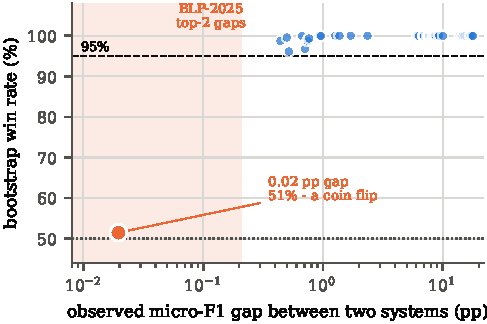
\includegraphics[width=\columnwidth]{fig3_gap_vs_winrate.pdf}
\caption{Bootstrap win rate against observed micro-F1 gap for all 45 pairs of
our ten systems. The only pair whose gap falls in the BLP-2025 range is a coin
flip (51.5\%). Every pair we could resolve reliably had a gap of at least
0.44\,pp.}
\label{fig:gapwin}
\end{figure}

\section{How Much Do Systems Actually Disagree?}
\label{sec:empirical}

The bound in \S\ref{sec:rankings} is only as good as its assumption about
discordance, so we measure it. We trained ten systems on the official train
split and evaluated each once on the official test split, varying feature space,
classifier family, regularisation, and class weighting---the axes along which
real submissions differ. Micro-F1 ranges 0.4984--0.6776; these are classical
models and do not reach the 0.7362 of the shared task's transformer ensembles
(see Limitations).

\paragraph{Measured discordance.} Across all 45 pairs, the two systems make
different predictions on a median of 32.0\% of items (range 4.4--48.5\%), and
McNemar's discordant cells $b+c$ cover a median of 25.5\% (range
3.6--36.3\%). Restricting to the ten pairs within 1\,pp of each other---the
regime the BLP leaderboard occupies---median discordance is still 8.8\%, or 895
items. \textbf{The lowest discordance we observed anywhere was 3.6\%, against
the ${<}0.8\%$ that Table~\ref{tab:mcnemar} shows would be required.}

\paragraph{Minimum detectable difference.} Inverting McNemar at each observed
discordance level gives the smallest gap that could be resolved
(Table~\ref{tab:mdd}). Even at our lowest observed discordance the minimum
detectable gap is 0.37\,pp; all three BLP top-two gaps (0.17, 0.21, 0.14\,pp)
fall below it.

\begin{table}[h]
\centering\small
\begin{tabular}{lrr}
\toprule
Discordance level & \% of $n$ & Min.\ gap \\
\midrule
lowest observed & 3.6 & 0.37 pp \\
median, near-tied pairs & 8.8 & 0.57 pp \\
median, all pairs & 25.5 & 0.98 pp \\
highest observed & 36.3 & 1.17 pp \\
\midrule
\multicolumn{2}{l}{\emph{BLP-2025 top-two gaps}} & 0.14--0.21 pp \\
\bottomrule
\end{tabular}
\caption{Smallest micro-F1 gap resolvable at $p<.05$, given observed
discordance. Every BLP top-two gap is below every threshold.}
\label{tab:mdd}
\end{table}

\paragraph{A necessary qualification.} Small gaps are not automatically
meaningless: our own top two differ by 0.44\,pp with only 4.1\% discordance and
hold their order in 98.7\% of 4{,}000 resamples. The defensible claim is
conditional---a gap is uninformative when smaller than $1.96\sqrt{b+c}/n$---so
what condemns the BLP gaps is their size \emph{relative to plausible
discordance}, not their size alone. Figure~\ref{fig:gapwin} shows the
transition: the one pair inside the BLP range wins 51.5\% of resamples, while
every pair we could resolve had a gap of at least 0.44\,pp.

\paragraph{Micro-F1 hides the systems that behave best.} Five of our ten systems
score exactly $0.000$ F1 on \textsc{Sexism}, detecting none of its 29 instances;
the best detects 3, for an F1 of 0.115. (Only one system never emits the label
at all; the others emit it but never correctly.) That best-performing system on
\textsc{Sexism} also has the best macro-F1, 0.5019---and ranks only
\emph{fourth} of ten on micro-F1. Micro and macro rankings agree weakly (Kendall
$\tau=0.467$, $p=.073$). Optimising the reported metric does not merely fail to
reward rare-class detection: in our pool it actively demotes the system that
does it best.

\section{Is Annotation Noise the Ceiling?}
\label{sec:ceiling}

A natural explanation for a plateau at 0.736 is that the labels themselves are
only that reliable. We test this and find it false.

From the reported $\kappa$ and the observed class marginals
($P_e=0.3887$), pairwise annotator agreement is $P_o = \kappa(1-P_e)+P_e =
0.823$. Modelling each annotator as correct with probability $\alpha$ and
otherwise mistaken, we solve for $\alpha$ under two error models: errors
scattered uniformly across the remaining classes, and errors maximally
correlated onto a single confusable class---the pessimistic case, since
correlated errors defeat majority voting. We then compute the probability that
the majority of three annotators recovers the true label.

\begin{table}[h]
\centering\small
\begin{tabular}{lcccc}
\toprule
Dimension & $\kappa$ & $P_o$ & $\alpha$ & Gold acc. \\
\midrule
Type      & 0.71 & 0.823 & .906\,/\,.902 & \textbf{.975\,/\,.973} \\
Target    & 0.79 & 0.872 & .933\,/\,.931 & .987\,/\,.986 \\
Severity  & 0.84 & 0.902 & .950\,/\,.948 & .993\,/\,.992 \\
\bottomrule
\end{tabular}
\caption{Estimated per-annotator accuracy $\alpha$ and majority-vote gold
accuracy, under uniform\,/\,correlated error models.}
\label{tab:ceiling}
\end{table}

Both models place the ceiling near 0.97 (Table~\ref{tab:ceiling}). Three-way
majority voting is strikingly effective at cleaning $\kappa=0.71$ annotations.
Against a best reported system of 0.7362, this leaves a gap of roughly 23.7
points that annotation noise does not explain. The plateau reflects genuine
modelling difficulty---or, as we argue next, a metric that stops rewarding
progress.

\begin{figure}[t]
\centering
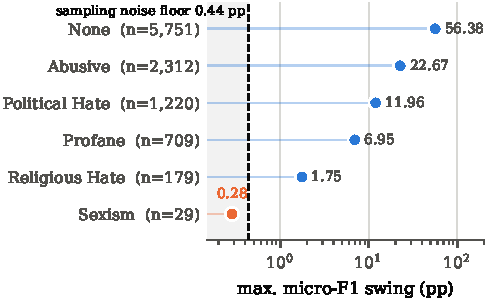
\includegraphics[width=\columnwidth]{fig2_metric_sensitivity.pdf}
\caption{The largest micro-F1 change any system can obtain by going from zero to
perfect recall on each class. \textsc{Sexism} falls below the sampling noise
floor: the metric cannot detect whether a system handles it at all.}
\label{fig:sensitivity}
\end{figure}

\section{What Can Micro-F1 Measure?}
\label{sec:metric}

At $n=10{,}200$ and $p\approx.735$, the sampling standard error of a single
micro-F1 score is 0.44 points. Because micro-F1 weights every item equally, the
maximum change any class can induce is bounded by its share of the test set.
Figure~\ref{fig:sensitivity} plots these bounds.

\textsc{Sexism} accounts for 29 of 10{,}200 test items. A system with perfect
recall on sexist content and a system that never predicts the class differ by at
most \textbf{0.28 points} of micro-F1---below one standard error, and smaller
than the 0.34-point spread separating the entire top five in 1A.
\textsc{Religious Hate} (179 items, 1.75 points) is only marginally better
placed.

For a hate-speech benchmark this is a design failure, not a statistical
curiosity: the evaluation offers no incentive to detect the categories most
plausibly tied to real-world harm, and cannot report whether any system does.
The majority baseline is 0.5638, so the measurable range above it is 17.2
points, of which \textsc{Sexism} occupies 1.6\%. Reporting macro-F1 alongside
micro-F1 would cost nothing and resolve this.

\section{Label-Schema Coherence}
\label{sec:coherence}

Subtask 1C labels type, severity, and target jointly, permitting internal
consistency checks (Table~\ref{tab:coherence}).

\begin{table}[h]
\centering\small
\begin{tabular}{lrr}
\toprule
Condition & $n$ & \% test \\
\midrule
type=None, severity$\neq$Little to None & 0 & 0.00 \\
type=None, target$\neq$None & 0 & 0.00 \\
type$\neq$None, \textbf{target=None} & \textbf{342} & \textbf{3.35} \\
type$\neq$None, severity=Little to None & 986 & 9.67 \\
\bottomrule
\end{tabular}
\caption{Internal consistency of subtask 1C test labels.}
\label{tab:coherence}
\end{table}

The 986 items combining a hate type with \textsc{Little to None} severity are a
\emph{tension} rather than an error: casual profanity may reasonably be
\textsc{Profane} with little hateful intent. The 342 bearing a hate type but no
target are harder to defend, since hostility aimed at nobody contradicts the
scheme. We flag these as the priority stratum for re-annotation rather than
counting them as confirmed errors.

\paragraph{The dataset is otherwise clean.} Across all 50{,}746 items we find
zero duplicate texts carrying conflicting labels, zero verbatim train/test
leakage, zero empty or sub-three-word items, and zero items lacking Bangla
script. Against the 52.8\% and 66.1\% error rates \citet{jin2026broken} report
for English text-to-SQL benchmarks, \textsc{BanglaMultiHate} is a markedly
better-constructed resource. Our criticism is of the evaluation, not the data.

\section{Recommendations}
\label{sec:disc}

\begin{enumerate}\itemsep0pt\parskip0pt
\item \textbf{Report confidence intervals.} One line of code; it would have
      shown these five-way ties immediately.
\item \textbf{Release per-system predictions,} without which McNemar is
      uncomputable outside the organising committee.
\item \textbf{Report macro-F1 alongside micro-F1} on skewed label
      distributions, so rare classes stay visible.
\item \textbf{Validate schema coherence at release.} Table~\ref{tab:coherence}
      is mechanical.
\item \textbf{Declare ties.} Ordering noise manufactures a false narrative of
      progress.
\end{enumerate}

\section{Conclusion}

The dataset is well constructed; the evaluation cannot support the rankings it
reports. The top five systems are tied in all three subtasks, the plateau is not
annotation noise, and the metric is blind to the rarest hate category.

\section*{Limitations}
\label{sec:limitations}

Our strongest claims (\S\ref{sec:rankings}) rest on published scores and the
released test set, and hold without further assumptions. Three limitations
qualify the rest.

First, we do not have the shared task's per-system predictions. \S\ref{sec:empirical}
substitutes ten systems of our own, but these are classical models spanning
0.4984--0.6776 micro-F1, below the 0.7362 of the transformer ensembles they stand
in for. Discordance between two strong transformers fine-tuned from the same
pretrained checkpoint could be lower than anything we measured, since they share
an initialisation our systems do not. We regard 3.6\% as an empirically grounded
floor rather than a proven one; obtaining the organisers' prediction files would
settle the question directly, and we invite them to release these. Second, the ceiling estimate in
\S\ref{sec:ceiling} assumes annotators err independently given the true label
and adopts a simplified two-parameter error model. Real annotator errors may be
correlated in ways neither model captures, which would lower the ceiling; we
report the pessimistic correlated-error variant alongside the uniform one, but
both remain models. Third, our coherence analysis (\S\ref{sec:coherence})
identifies items whose labels are mutually inconsistent, which is not the same
as identifying which of the labels is wrong. Resolving that requires the manual
re-annotation stage this paper does not yet report: a 495-item stratified sample,
three blind annotators, and the C0--C4 difficulty taxonomy adapted from
\citet{jin2026broken}. Finally, this audit covers one shared task in one
language and does not establish how common these patterns are.

\section*{Ethics Statement}

This work analyses an existing, publicly released dataset of hate speech under
its CC BY-NC-SA 4.0 licence; we redistribute no data, only analysis code. We
name teams only as they appear in the published overview paper, and our findings
are not criticisms of those teams: the systems may well differ in quality, and
our point is precisely that the evaluation cannot tell us. We note that a metric
insensitive to sexist content risks under-serving those most affected by it,
which motivates \S\ref{sec:metric}.

We thank the BLP-2025 organisers, whose decision to release data, gold labels,
and scorer is what made this audit possible; we would encourage other shared
tasks to match that standard.

\bibliography{refs}
\bibliographystyle{acl_natbib}

\end{document}
